\documentclass[11pt]{article}
\usepackage[letterpaper,margin=0.87in]{geometry}
\usepackage{amsmath,amssymb,booktabs,graphicx,microtype,xcolor}
\usepackage{listings}
\usepackage[colorlinks=true,linkcolor=black,urlcolor=teal]{hyperref}
\setlength{\parindent}{0pt}
\setlength{\parskip}{0.62em}
\definecolor{accent}{HTML}{176C61}
\definecolor{codebg}{HTML}{F5F7F7}
\definecolor{codeborder}{HTML}{D5E1DF}
\definecolor{codecomment}{HTML}{52605D}
\lstdefinestyle{sircode}{
  language=Python,
  basicstyle=\small\ttfamily,
  keywordstyle=\color{accent}\bfseries,
  commentstyle=\color{codecomment},
  backgroundcolor=\color{codebg},
  rulecolor=\color{codeborder},
  frame=single,
  framesep=6pt,
  xleftmargin=6pt,
  xrightmargin=6pt,
  columns=fullflexible,
  keepspaces=true,
  showstringspaces=false
}
\newcommand{\reportsection}[1]{\section*{\textcolor{accent}{#1}}}

\begin{document}
{\small\textcolor{accent}{STA492 \enspace / \enspace SIMULATION-BASED INFERENCE}\par}
{\LARGE\bfseries Inferring transmission and recovery\\[2pt] from three SIR maps\par}
\vspace{0.35em}
We estimate two probabilities from three snapshots of a simulated outbreak.
The experiment asks what we gain by tracking \emph{who} stays infectious,
in addition to counting \emph{how many} are infectious.

\reportsection{1. The simulator and the observed data}

The presentation uses a $24\times24$ grid with four infectious people in the
center at time zero. All other cells start susceptible. A cell has neighbors
above, below, to its left, and to its right where those cells exist. Let
$p$ be the probability of transmission from one infectious neighbor, and $q$
the probability of recovery in one step. When a susceptible person has $k$
infectious neighbors, all $k$ transmission attempts fail with probability
$(1-p)^k$. Thus
\[
\Pr(S\longrightarrow I\mid k)=1-(1-p)^k,\qquad
\Pr(I\longrightarrow R)=q.
\]
The simulator computes new infections and recoveries from the current grid
before updating any cell. Recovered people stay recovered. The visits report
only whether each person is currently infectious. We use the presentation's
maps, generated at $(p,q)=(0.41,0.18)$ with seed 917. These values serve as a
check after inference.

\noindent\makebox[\linewidth]{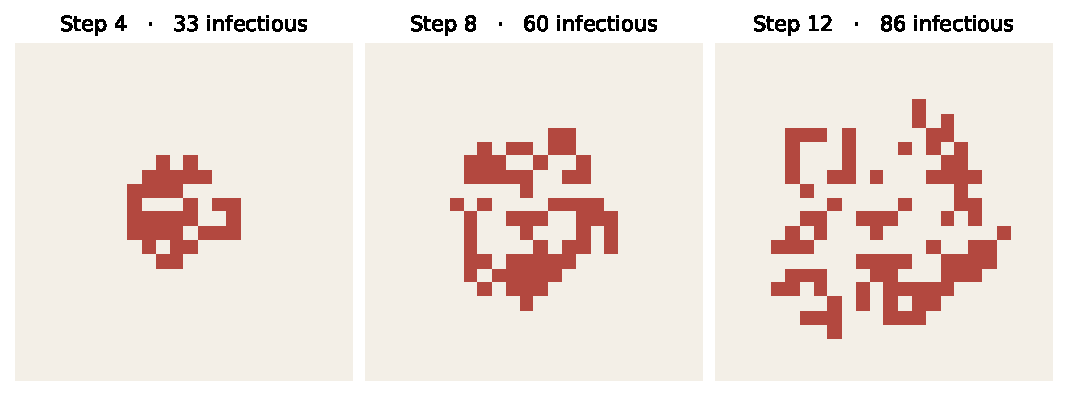
\includegraphics[width=0.72\linewidth]{results/observed_maps.pdf}}\par
\vspace{-0.5em}

\reportsection{2. Compressing the maps}

Let $Y_t(v)$ indicate whether person $v$ is infectious at visit $t$. The count
$C_t$ measures the size of the infectious population. The overlap $O_{t,t+4}$
counts people infectious at both visits.
\[
C_t=\sum_vY_t(v),\qquad O_{t,t+4}=\sum_vY_t(v)Y_{t+4}(v),\qquad
s^*=(33,60,86,17,25).
\]
The first three entries are the counts at $4,8,12$. The last two entries are
the overlaps for $4$ to $8$ and $8$ to $12$. Conditional on the grid at $t$,
each of the $C_t$ infectious people remains infectious at $t+4$ if they avoid
recovery on four successive steps. Their recovery draws are independent, so
\[
O_{t,t+4}\mid Y_t,p,q\sim \operatorname{Binomial}\bigl(C_t,(1-q)^4\bigr).
\]
Pooling the observed overlaps gives a rough recovery estimate of
$1-[(17+25)/(33+60)]^{1/4}\approx0.180$. This uses retention alone. The
neural estimator uses the joint distribution of counts and overlaps.

\newpage
\reportsection{A visual walkthrough of the summaries}

\textbf{Count the red cells, then match the same cells across visits.}
The first two panels show the actual observations at steps 4 and 8. In
the overlay, purple marks the cells that were red on both maps. Counting
just those cells gives the overlap of 17.

\begin{figure}[!ht]
\centering
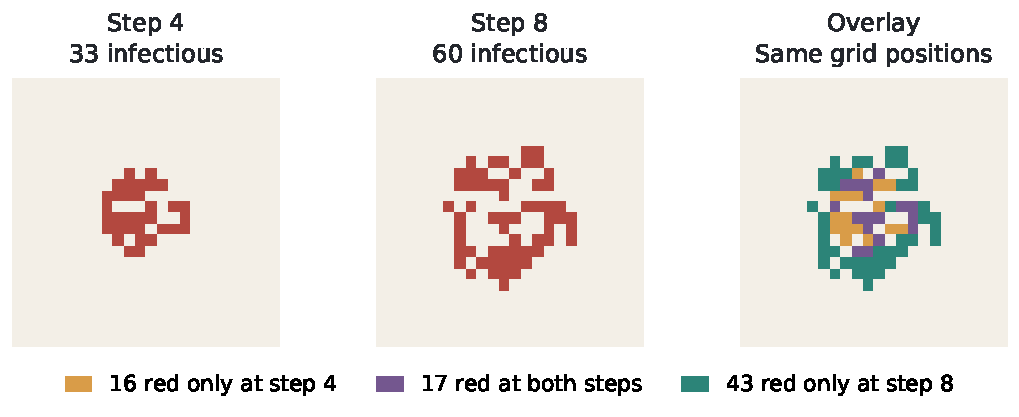
\includegraphics[width=0.92\linewidth]{results/summary_overlap.pdf}
\caption{Of the 33 people infectious at step 4, 17 are still infectious
at step 8 and 16 have recovered. The 43 people red only at step 8 became
infectious after step 4 and are still infectious at step 8.}
\end{figure}

Repeating the overlay for steps 8 and 12 gives 25. These five numbers are
all the observation inputs to the summary model.
\[
\text{Three maps}
\quad\longrightarrow\quad
\bigl(\underbrace{33,60,86}_{\text{counts}},\
      \underbrace{17,25}_{\text{overlaps}}\bigr)
\quad\longrightarrow\quad
\text{posterior for }(p,q).
\]

\textbf{The summaries leave out where infections are clustered.}
In the illustration below, imagine repeating each pattern at all three
visits. Both examples give counts of $(4,4,4)$ and overlaps of $(4,4)$.

\begin{figure}[!ht]
\centering
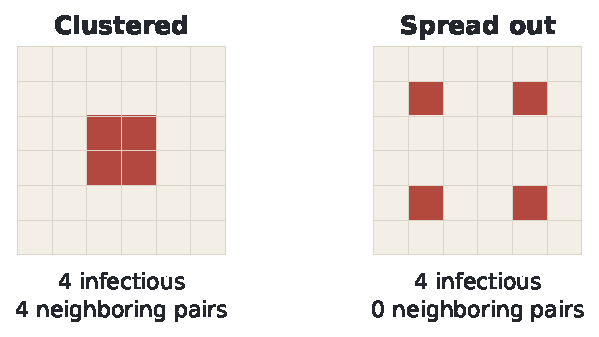
\includegraphics[width=0.55\linewidth]{results/summary_spatial_loss.pdf}
\caption{Two schematic grids with the same five summaries. A neighboring
pair is two infectious cells that share a side. The block on the left
has four such pairs, and the map on the right has zero.}
\end{figure}

\newpage
\reportsection{3. Learning the posterior with simulations}

Write $\theta=(p,q)$ and let $\pi$ denote the prior and the posteriors under
the simulator. We draw $p,q$ independently from $\operatorname{Uniform}(0,1)$.
For each $\theta_i$, simulate an outbreak and summarize the same three visits
to obtain $s_i$. We use 36{,}000 simulations for training, 4{,}000 for
validation, and 4{,}000 for testing. Both fits use the same parameter draws and
the same outbreaks. One receives just the counts and the other receives all
five summaries. Their inputs are $\log(1+s_i)$, then standardized using the
training set. We hold the presentation maps apart from these simulations.

\textbf{Why neural posterior estimation (NPE)?}
We want a joint density for two parameters from a short vector. A conditional
flow lets us draw from that density directly for any new summary. Neural
likelihood estimation would require a model of the summaries given $\theta$
and a separate step to sample the posterior. We use NPE here for its direct
sampling and low-dimensional output \cite{npe}.

For each training pair, we reward high density at the generating parameters
by minimizing
\[
-\frac{1}{N}\sum_{i=1}^{N}\log f_\phi(\theta_i\mid s_i).
\]
For a fixed summary $s$, adding and subtracting $\log \pi(\theta\mid s)$
inside its population expectation gives
\[
\mathbb E_{\theta\mid s}\!\left[-\log f_\phi(\theta\mid s)\right]
=
\underbrace{\mathbb E_{\theta\mid s}[-\log\pi(\theta\mid s)]}_{\text{constant in }\phi}
+
D_{\mathrm{KL}}\bigl(\pi(\cdot\mid s)\,\|\, f_\phi(\cdot\mid s)\bigr).
\]
Averaging over $s$ gives the objective that the simulated training pairs
approximate. The target is the posterior given the summaries. Spatial
arrangement and unobserved infection times are outside those summaries.

\textbf{How the flow computes a density.}
Start with $z\sim N(0,I_2)$. In one layer, keep $u_1$ and send
$u_2\mapsto u_2e^{a(u_1,s)}+b(u_1,s)$. A small network computes $a$ and $b$.
The Jacobian is triangular, so the layer's forward log determinant is $a$.
It is invertible because the scale $e^a$ is positive and $u_1$ is available
when reversing the layer. We use six layers that alternate the kept
coordinate, as in Real NVP \cite{realnvp}. The last map takes the two output
coordinates $u$ to $\theta_j=\sigma(u_j)$, where $\sigma$ is the sigmoid.
On the way back, $u_j=\log[\theta_j/(1-\theta_j)]$ and
$du_j/d\theta_j=1/[\theta_j(1-\theta_j)]$. If $T_s$ denotes the entire
forward map, the learned density on the unit square is
\[
\log f_\phi(\theta\mid s)
=\log\varphi_2\bigl(T_s^{-1}(\theta)\bigr)
 +\log\left|\det D_\theta T_s^{-1}(\theta)\right|.
\]
Here $\varphi_2$ is the standard bivariate normal density. The inverse log
determinant is the sum of the inverse contributions from the six couplings
and the sigmoid. Training uses Adam and restores the weights with the best
validation loss.

This experiment uses hand-chosen summaries. For related work on
\emph{learning} summaries, Wang and Onnela compress individual test results
and use them in ABC for a partially observed SIR model on a contact
network \cite{wang}.

\newpage
\reportsection{4. What did the overlaps add?}

The table gives posterior means from 8{,}000 draws per fit. Brackets give
the 5th and 95th percentiles for each parameter separately.

\begin{center}
\begin{tabular}{lcc}
\toprule
Input & Transmission $p$ & Recovery $q$\\
\midrule
Counts only & $0.874\ [0.637,\,0.992]$ & $0.489\ [0.374,\,0.556]$\\
Counts and overlaps & $0.422\ [0.366,\,0.483]$ & $0.181\ [0.146,\,0.224]$\\
\bottomrule
\end{tabular}

\vspace{0.35em}
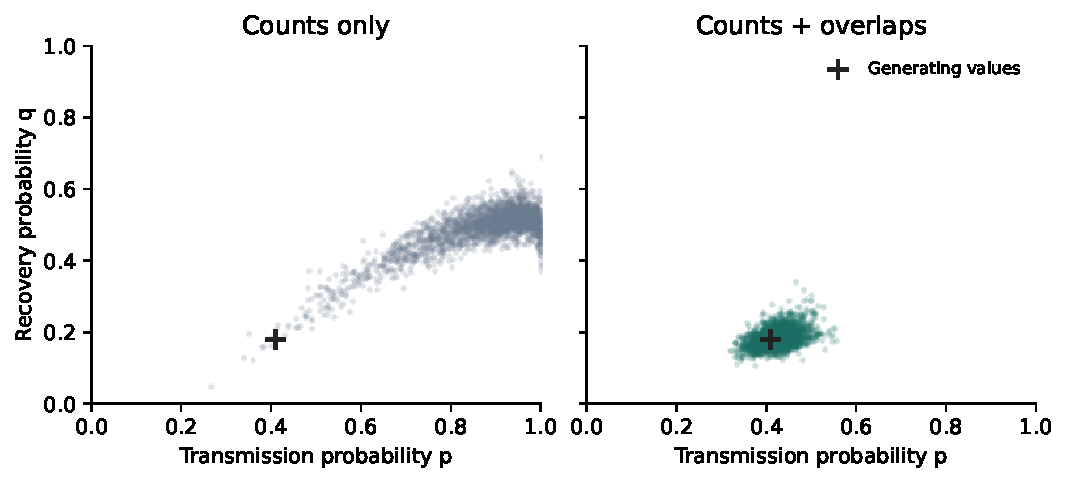
\includegraphics[width=0.73\linewidth]{results/posterior.pdf}
\par{\small Posterior draws. The cross marks the generating parameters.}
\end{center}

The counts-only model favors fast transmission and fast recovery. Such
outbreaks can have the right number of infectious people with much faster
turnover. Overlaps favor longer infectious periods and move both posterior
means toward the values used in the presentation.

On 4{,}000 independent test outbreaks, mean joint log density at the true
parameters was $2.209$ using counts and $2.911$ using both summaries. The
paired gain was $0.702$ nats per outbreak (Monte Carlo SE $0.016$).
Marginal 90\% intervals covered the true $p,q$ in 88.7\%, 90.8\% of 1{,}000
test cases for counts, and 90.0\%, 89.9\% with overlaps. These are averages
over the simulated prior and support using overlaps for this example.

We also simulated 1{,}500 new outbreaks from each fitted posterior. With
counts alone, the two overlap intervals were $[0,5]$ and $[1,10]$.
Adding overlaps shifted them to $[4,15]$ and $[11,33]$, compared with the
observed 17 and 25. The first count and first overlap still sit above
their central 90\% predictive intervals. This check compares new outbreaks
to one particular realization. The notebook plots all five predictive
intervals and reports the held-out checks separately.

\newpage
\reportsection{5. How do the summaries compare with the raw maps?}

The CNN learns 16 features from the three binary maps. Direct NPE
flattens the maps into 1{,}728 binary entries and passes them to the flow.
Within each training budget the models shared the training and validation
outbreaks, and both budgets used the same 4{,}000 test outbreaks.

\begin{figure}[!ht]
\centering
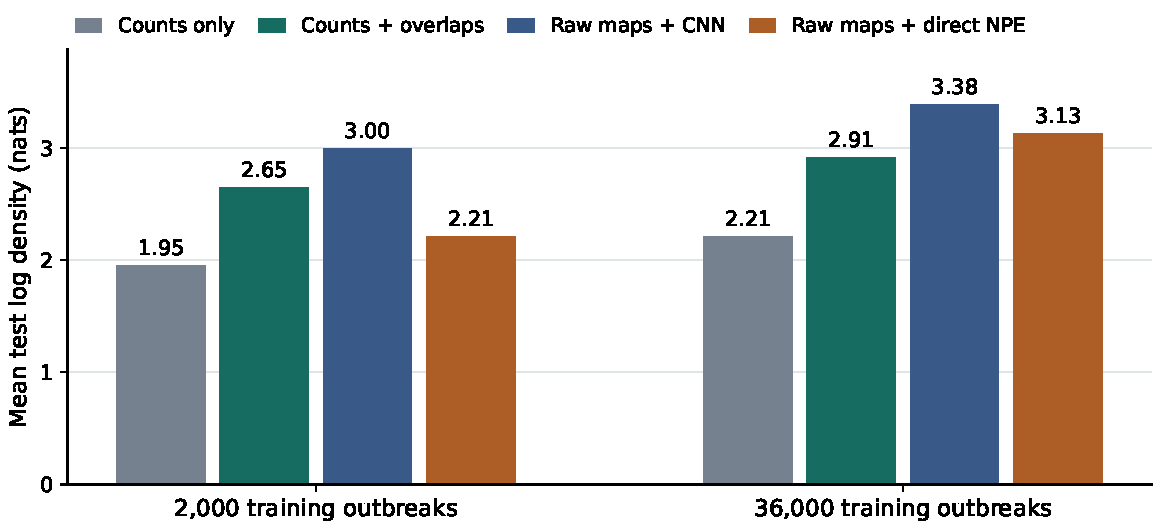
\includegraphics[width=0.92\linewidth]{results/summary_comparison.pdf}
\caption{Average log density assigned to the true parameter pair $(p,q)$
over the 4{,}000 test outbreaks. Higher is better. All four models were
evaluated at both training budgets.}
\label{fig:raw-map-comparison}
\end{figure}

\begin{figure}[!ht]
\centering
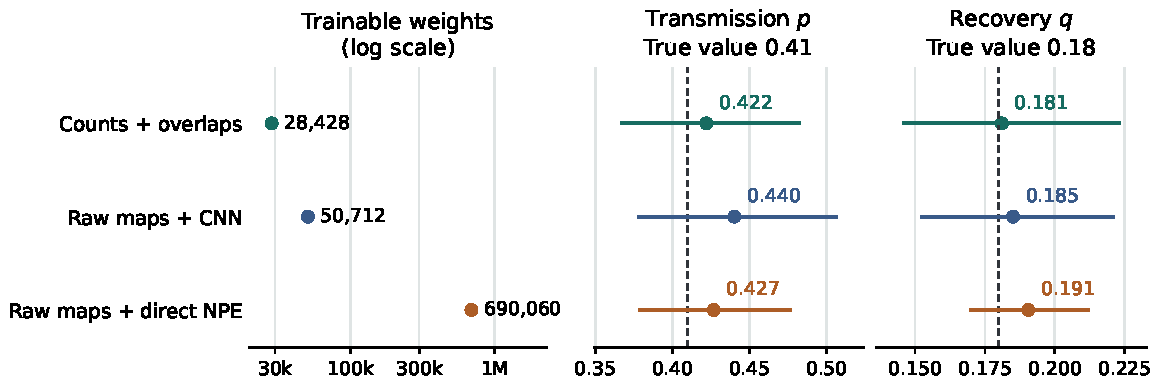
\includegraphics[width=0.99\linewidth]{results/summary_tradeoff.pdf}
\caption{Models trained on 36{,}000 outbreaks. The left panel shows
weight counts on a log scale. The other panels show posterior means and
marginal 90\% intervals for the presentation outbreak. Dashed lines mark
the generating values.}
\label{fig:summary-tradeoff}
\end{figure}

With 2{,}000 training outbreaks, overlaps raised the score from 1.95 to 2.65,
ahead of direct NPE at 2.21. At 36{,}000, direct NPE scored 3.13 versus
2.91 with counts and overlaps. The CNN scored highest at both budgets.
Direct NPE uses 690{,}060 weights because each coupling layer receives
the entire grid vector.

\newpage
\reportsection{6. Can we tell the posterior draws apart?}

For each of the 4{,}000 test outbreaks we make two pairs. The first is
$(x_i,\theta_i)$, the maps and the parameter pair that generated them.
The second is $(x_i,\widehat\theta_i)$, the same maps and one draw from
the fitted posterior. A correct posterior gives these pairs the same
joint distribution across outbreaks.

\textbf{Classifier two-sample test (C2ST).}
A separate classifier tries to identify the source of each pair
(\href{https://arxiv.org/abs/1610.06545}{Lopez-Paz and Oquab}).
It sees the parameter pair, counts and overlaps, and counts in
$4\times4$ blocks of each map. We train it on both rows from 2{,}000
outbreaks and measure its accuracy on the other 2{,}000. Both rows for
an outbreak stay on the same side of the split.

\begin{figure}[!ht]
\centering
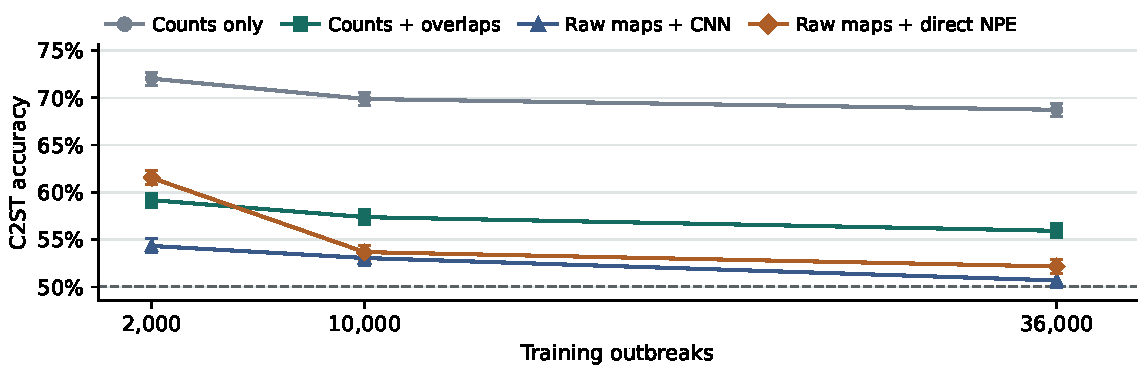
\includegraphics[width=0.96\linewidth]{results/c2st_comparison.pdf}
\caption{C2ST accuracy at 2{,}000, 10{,}000, and 36{,}000 training outbreaks.
The dashed line marks 50\% chance accuracy. Whiskers show one standard
error. The 10{,}000-outbreak fits use the 2{,}000-run training settings.}
\end{figure}

\textbf{Maximum mean discrepancy (MMD).}
We compare the pairs using Gaussian similarities on both the full maps
and the two parameters
(\href{https://www.jmlr.org/papers/v13/gretton12a.html}{Gretton et al.}).
We set the similarity scales from the validation outbreaks and omit terms
that compare an outbreak with itself. This estimates squared MMD while
accounting for the paired maps.

\begin{figure}[!ht]
\centering
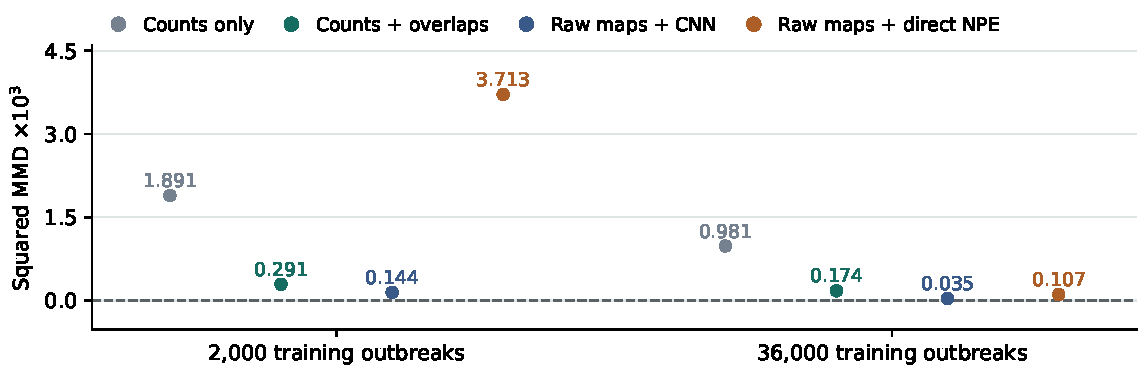
\includegraphics[width=0.96\linewidth]{results/mmd_comparison.pdf}
\caption{Squared MMD on the same 4{,}000 outbreaks, multiplied by
$10^3$ for readability. Zero is the reference value. The finite-sample
estimate can be slightly negative.}
\end{figure}

All four C2ST lines move toward 50\% across the measured budgets. Direct
NPE makes its largest drop by 10{,}000, and the CNN is closest to chance
at each budget. Adding overlaps improves C2ST at all three budgets and
squared MMD at the two shown.

\newpage
\reportsection{Appendix. Comparing the code paths}

The full benchmark is in \nolinkurl{simulations/sir/compare_raw_grid.py}.
These excerpts show what each model does with a batch of outbreaks.
Each row of \texttt{theta\_batch} contains the true $(p,q)$ that simulated
the corresponding maps.

\textbf{With summary statistics.}
The simulator gives three binary maps per outbreak. We compute counts
and overlaps first. The five columns form the input to the flow after
a log transform and standardization using the training set.

\begin{lstlisting}[style=sircode]
values = summarize(maps)  # shape: (batch_size, 5)
summary_input = torch.from_numpy(np.log1p(values).astype(np.float32))
log_density = summary_flow.log_prob(theta_batch, summary_input)
\end{lstlisting}

\textbf{With a CNN.}
The three visits are the input channels of the CNN. Its filters look at
small patches of cells. Training learns how to turn those patches into
16 features for the flow. The body of \texttt{RawGridNPE.log\_prob}
contains the two steps below.

\begin{lstlisting}[style=sircode]
# maps has shape (batch_size, 3, 24, 24)
features = self.encoder(maps.float())  # shape: (batch_size, 16)
return self.flow.log_prob(theta, features)
\end{lstlisting}

\textbf{With direct NPE.}
Reshaping keeps each binary entry in a fixed order. The flow receives all
1{,}728 entries directly.

\begin{lstlisting}[style=sircode]
pixels = maps.flatten(start_dim=1).float()  # (batch_size, 1728)
log_density = direct_flow.log_prob(theta_batch, pixels)
\end{lstlisting}

\textbf{Same training rule and test score.}
Training minimizes the negative mean of the log densities. On the test
set we average the log densities directly, so a higher score is better.
Here \texttt{inputs} holds the test data in the shape each model expects.
The function \texttt{score\_outbreaks} returns one value per test outbreak.

\begin{lstlisting}[style=sircode]
loss = -log_density.mean()  # Training
test_scores = score_outbreaks(model, theta, inputs, test_indices)
mean_test_log_density = test_scores.mean().item()
\end{lstlisting}

Figure~\ref{fig:raw-map-comparison} compares the scores. From
\nolinkurl{simulations/sir}, run the command below for direct NPE. Use
\texttt{2000} for the smaller run or \texttt{--model cnn} for the CNN.

\begin{lstlisting}[style=sircode,language={}]
python compare_raw_grid.py --model direct --training-outbreaks 36000
\end{lstlisting}

\begin{thebibliography}{3}
\small
\setlength{\itemsep}{0pt}
\bibitem{npe} G. Papamakarios and I. Murray (2016).
\href{https://proceedings.neurips.cc/paper/2016/hash/6aca97005c68f1206823815f66102863-Abstract.html}{Fast $\varepsilon$-free inference of simulation models with Bayesian conditional density estimation}.
NeurIPS.
\bibitem{realnvp} L. Dinh, J. Sohl-Dickstein, and S. Bengio (2017).
\href{https://arxiv.org/abs/1605.08803}{Density estimation using Real NVP}. ICLR.
\bibitem{wang} M. H. Wang and J.-P. Onnela (2024).
\href{https://doi.org/10.1093/comnet/cnae017}{Flexible Bayesian inference on partially observed epidemics}. \emph{Journal of Complex Networks}, 12(2).
\end{thebibliography}
\end{document}
